%============================================================================
%  QDOA — corrected manuscript for IEEE TETC
%  Compile: pdflatex (IAST transliteration, compiles anywhere).
%  To restore Devanagari surface forms: switch to xelatex/lualatex, add
%     \usepackage{fontspec}\newfontfamily\dev{Noto Sans Devanagari}
%  and wrap Devanagari spans in {\dev ...}.  All linguistic examples below
%  are given in IAST so the source is engine-independent.
%
%  HONEST-REPORTING NOTE (read before submitting):
%   - The morphology accuracy numbers in Table IV are from a CLEAN retrain of
%     the released code on the Aer simulator; they REPLACE the earlier
%     "96.0% / 96.0% identical, zero regression" claim, which did not survive
%     retraining.  The quantum Grover+PQC path shows a measurable regression.
%   - Table VII is the author's MEASURED ibm_marrakesh run (released code, n=4-9,
%     truncated by an account usage limit). Table VIII is the earlier ibm_fez run
%     (n=4-12) that reaches the noise wall. Insert real job IDs / calibration
%     dates where marked "% TODO: job id"; hardware runs are not seed-reproducible.
%     Re-run ibm_marrakesh n=10..12 (pinned backend) when usage resets.
%   - Morphology accuracy (Table IV) is the K=20 controlled variance study
%     (run_variance.py): quantum NISQ 93.3+/-5.5% IV, 82.0+/-7.6% OOV, training-
%     driven (ideal and NISQ means coincide). It is a distribution, not one run.
%   - Bibliography entries marked "% VERIFY" were reconstructed from the draft
%     PDF text; check each against your master .bib before submission.
%============================================================================
\documentclass[journal]{IEEEtran}

\usepackage{amsmath,amssymb}
\usepackage{booktabs}
\usepackage{array}
\usepackage{graphicx}
\usepackage{xcolor}
\usepackage{multirow}
\usepackage{url}
\usepackage{tikz}
\usetikzlibrary{shapes.geometric,arrows.meta,positioning,fit,backgrounds}
\usepackage{pgfplots}
\pgfplotsset{compat=1.17}
\usepgfplotslibrary{groupplots}
\usepackage[ruled,vlined]{algorithm2e}
\usepackage{qcircuit}
\usepackage[hidelinks]{hyperref}
\usepackage{csquotes}
% DOIs in the references (IEEEtranDOI.bst writes \doi{...}): roman type, linked
\urlstyle{same}
\providecommand{\doi}[1]{\href{https://doi.org/#1}{\nolinkurl{#1}}}

\newcommand{\bigO}{\mathcal{O}}
\newcommand{\sqrtN}{\sqrt{N}}
\providecommand{\ket}[1]{\ensuremath{|#1\rangle}}
\providecommand{\bra}[1]{\ensuremath{\langle#1|}}

\begin{document}

\title{Quantum Dynamic Oracle Adaptation for Multilingual Indian Morphological
Analysis: Hardware-Aware Grover Search and an Honestly Reported Accuracy--Query
Trade-off on IBM Heron}

\author{
\IEEEauthorblockN{
$^1$,$^2$Prasad Patil
}\\
\IEEEauthorblockA{
$^1$Department of Computer Science and Engineering\\
Indian Institute of Information Technology Nagpur, India $-$ 441108\\
dtei24cse008@iiitn.ac.in
} \\
\IEEEauthorblockA{
$^2$Tata Consultancy Services, Nagpur, India\\
p.ppatil@tcs.com
}}

\maketitle

\begin{abstract}
India records 121 mother tongues, with 26\% of the population bilingual and
7.1\% trilingual; in Maharashtra, home to 83~million Marathi speakers,
bilingualism reaches 51.1\%. Morphological analysis underpins downstream NLP
for these languages, yet classical analyzers use $\bigO(N)$ sequential search
over candidate segmentations. Existing Quantum NLP systems (DisCoCat, lambeq)
target compositional \emph{sentence} semantics in English; to our knowledge no
prior work applies quantum search to \emph{morphological} segmentation of
Sanskrit, Marathi, or any Indian language. We present QDOA, the first
quantum-search morphological analyzer for multilingual Indian NLP, built on the
Dynamic Oracle Adaptation paradigm. QDOA pairs Grover amplitude amplification
with a grammar oracle and a 3-qubit parameterised quantum circuit (PQC) for
few-shot out-of-vocabulary (OOV) inference. Our contributions are primarily
\emph{methodological and hardware-side}: (i) a hardware-aware Grover protocol
(v-chain MCX with clean ancillas, XY4 dynamical decoupling, gate/measurement
twirling, trial transpilation, an empirical iteration sweep, and a $k{=}0$
no-amplification control that turns the noise wall from an asserted into a
\emph{measured} quantity); and (ii) three-counter honest oracle accounting that
separates classical grammar evaluations from quantum circuit executions.
On MorphoQ-131 (a curated 131-sample trilingual dataset), classical beam search
attains a deterministic 100.0\% Top-1 in-vocabulary and 86.7\% OOV accuracy. Over
$K{=}20$ independent PQC trainings the quantum Grover+PQC path averages
$93.3\pm5.5\%$ in-vocabulary and $82.0\pm7.6\%$ OOV---a modest deficit below the
classical baseline that is \emph{training-driven, not noise-driven} (the noiseless
and NISQ means coincide within one standard deviation), with the best trainings
reaching parity. Motivated by this, we introduce a \emph{scoring oracle} that
replaces mark-only amplification with a quantum maximum-finding (D\"urr--H\o yer)
selection subroutine: on the same benchmark it cuts in-vocabulary run-to-run
variance roughly five-fold ($\pm5.5\%\!\to\!\pm1.1\%$) and lifts OOV accuracy to
$88.0\%$, matching or exceeding the classical baseline, at $\bigO(\sqrtN)$ query
cost. We locate the quantum path's benefit in asymptotic query
complexity---$\bigO(\sqrtN)$ oracle queries versus $\bigO(N)$---with a structural
crossover projected at $n\!\ge\!8$. In a separate experiment characterising the
Grover primitive itself, a single-device \texttt{ibm\_fez} (Heron~r2) run over
$n{=}4$--$12$ locates the noise wall at $n\!\ge\!11$ by a binomial test against a
$k{=}0$ control, corroborated by a truncated run of the released code on
\texttt{ibm\_marrakesh} ($n{=}4$--$9$, median two-qubit gate error
$2.8\times10^{-3}$) showing 100\% success through $n{=}7$, 98\% at $n{=}8$, 90\%
at $n{=}9$, all significant against the control ($p<10^{-3}$). On both devices the
empirically optimal Grover iteration count is $k{=}1$ across the usable regime,
consistent with recent Heron-family reports.
\end{abstract}

\begin{IEEEkeywords}
Grover search, amplitude amplification, hardware-aware quantum protocols,
noise-wall characterization, dynamical decoupling, Pauli twirling, Indian
multilingual NLP, Sanskrit/Marathi morphology, honest oracle accounting,
parameterised quantum circuits, MorphoQ-131, QNLP, NISQ, IBM Heron.
\end{IEEEkeywords}

\section{Introduction}

\subsection{The Indian Multilingual Context}
The 2011 Census documents 121 mother tongues and 22 scheduled languages, with
26\% of the population bilingual~\cite{census2011}. Educated speakers routinely
navigate a mother tongue, Hindi or a regional contact language, and English,
and many share Sanskrit-derived vocabulary across Hindi (528~million speakers),
Marathi (83~million), and other Indo-Aryan languages~\cite{ethnologue2023}.
Morphological analysis---decomposing a surface word into stem and affixal
morphemes---is foundational to parsing, machine translation, and information
retrieval~\cite{goldberg2017,bharati1995}. Indo-Aryan languages are richly
inflectional: a single Sanskrit nominal stem generates dozens of case-number
forms, Marathi layers postpositions and oblique stems over a nominal base, and
morphophonemic sandhi mutates the surface at the morpheme boundary, so the
mapping from surface string to (stem, suffix) is genuinely a \emph{search} over
competing analyses rather than a lookup. For a word of length $L$, up to
$L\!-\!1$ candidate segmentations must each be grammatically validated; padded to
a power of two for quantum indexing this yields a search space of $N=2^{n}$, over
which classical beam search incurs $\bigO(N)$ oracle calls. This structure---a
uniform, unstructured search over candidate parses gated by a Boolean grammar
predicate---is exactly the setting in which Grover amplitude amplification offers
an asymptotic $\bigO(\sqrtN)$ query advantage, which motivates casting
morphological segmentation as a quantum search problem. Whether that asymptotic
advantage survives to useful accuracy on present-day noisy hardware is the
empirical question this paper answers, honestly and in both directions.

\subsection{Scope, and an Honest Statement of What This Paper Does and Does Not
Show}
This paper makes three kinds of claim, kept strictly separate.
\emph{(1) An end-to-end morphology system} on a noisy simulator
(Sections~\ref{sec:pipeline}--\ref{sec:morphbench}): the mark-only Grover+PQC path
does \textbf{not} robustly match classical accuracy---over $K{=}20$ trainings it
averages a $\sim$7-point IV deficit with a wide, training-driven spread---so its
justification is asymptotic query complexity, not accuracy. \emph{(2) A scoring
oracle} (Section~\ref{sec:scoring}) that fixes this: a quantum maximum-finding
selection cuts the variance $\sim$5$\times$ and lifts OOV to/above the classical
baseline, still on a (device-calibrated) simulator, not real hardware.
\emph{(3) A hardware characterisation of the Grover primitive}
(Section~\ref{sec:hwbench}) on \texttt{ibm\_fez}/\texttt{ibm\_marrakesh} over
\emph{random} marked states, isolating how deep an amplification circuit the
protocol sustains and certifying, via a $k{=}0$ control and binomial test, where
amplification remains significant. We label every result with the experiment it
belongs to, and make no present-day end-to-end quantum-advantage claim.

\subsection{Limitations up Front}
Three limitations bound every claim and are expanded in
Section~\ref{sec:limitations}: MorphoQ-131 is small (131 samples, 90 evaluation
words), the Stage-1 grammar oracle's linguistic content is specified classically
(QDOA is quantum \emph{search} over a classical oracle), and the full pipeline is
demonstrated in simulation, not yet on real hardware.

\subsection{Contributions}
\begin{enumerate}
\item A \textbf{hardware-aware Grover protocol} (Section~\ref{sec:protocol})
combining v-chain MCX with clean ancillas, XY4 dynamical decoupling,
gate/measurement Pauli twirling, five-seed trial transpilation, an empirical
iteration sweep, and---critically---a $k{=}0$ no-amplification control that,
with a one-sided binomial test, certifies where amplification is significant.
\item \textbf{Three-counter honest oracle accounting}
(Section~\ref{sec:accounting}) that removes two biases we identify in prior
QNLP reporting: oracle-counter pollution and unit mismatch between classical
grammar evaluations and quantum circuit runs.
\item \textbf{MorphoQ-131} (Section~\ref{sec:dataset}), the first curated
trilingual (English/Sanskrit/Marathi) quantum morphological benchmark, released
openly, with an enforced surface-reconstructability invariant.
\item An \textbf{honest accuracy--query characterisation}
(Section~\ref{sec:morphbench}): the classical path is deterministic
(100.0\%/86.7\%); over $K{=}20$ trainings the quantum path averages
$93.3\pm5.5\%$ IV and $82.0\pm7.6\%$ OOV, a modest, training-driven (not
noise-driven) deficit, so we report its distribution and locate its benefit in
query complexity.
\item A \textbf{scoring oracle via quantum maximum-finding}
(Section~\ref{sec:scoring}) that replaces mark-only amplification with a
D\"urr--H\o yer selection subroutine, cutting in-vocabulary variance
$\sim$5$\times$ ($\pm5.5\%\!\to\!\pm1.1\%$) and lifting OOV accuracy to/above the
classical baseline at $\bigO(\sqrtN)$ query cost, with comparisons to standard
classical baselines (longest-match, productive-suffix).
\item A \textbf{single-device hardware certification}
(Section~\ref{sec:hwbench}) of Grover amplitude amplification on \texttt{ibm\_fez}
across $n{=}4$--$12$, locating the noise wall at $n\!\ge\!11$ by the $k{=}0$
binomial test, corroborated by a released-code run on \texttt{ibm\_marrakesh}
($n{=}4$--$9$), with an empirical $k{=}1$ finding on both devices.
\end{enumerate}

\section{Related Work and Positioning}

\subsection{Quantum Search and Near-Term Computing}
Grover search~\cite{grover1996} and its tight iteration
bounds~\cite{bbht1998} provide a quadratic speedup for unstructured
search and underlie many quantum subroutines~\cite{nielsen2010}. In the noisy
intermediate-scale quantum
(NISQ) regime~\cite{preskill2018}, however, deep amplitude amplification is
limited by two-qubit error accumulation, and empirical studies report that the
success-maximising iteration count falls below the textbook
optimum~\cite{morales2018,mandviwalla2018}. Recent hardware demonstrations have
shown pre-fault-tolerant utility on superconducting
processors~\cite{kim2023}, and application-oriented benchmarking suites now
characterise such devices systematically~\cite{preston2022,lubinski2023}.
Quantum-inspired and emerging-computing accelerators for the same search and
optimisation workloads---for example, FPGA-based simulated annealers---define the
classical frontier our $\bigO(N)$ baseline abstracts~\cite{waidyasooriya2021}.
Our Dynamic Oracle Adaptation line~\cite{doa2026} sits in this space; the present
work extends it from parameter estimation to morphological search with an
explicit $k{=}0$-referenced noise-wall test.

\subsection{Quantum NLP and Machine Learning}
Compositional QNLP---DisCoCat~\cite{coecke2020qa} and lambeq~\cite{lambeq2021},
with foundations~\cite{coecke2020found}, early algorithms~\cite{zeng2016}, and
hardware demonstrations~\cite{lorenz2023,meichan2021}---encodes \emph{sentence}%
-level grammatical structure and has been run on quantum hardware for
classification and question answering; variational circuits have also been used
for topic modelling~\cite{qiao2024}. More broadly, quantum machine
learning~\cite{biamonte2017} with quantum-enhanced feature
spaces~\cite{havlicek2019,schuld2019} and parameterised quantum circuits (PQCs)
trained variationally~\cite{mitarai2018,benedetti2019,cerezo2021}
forms the basis of our Stage-3 few-shot learner, subject to the trainability
caveats of barren plateaus~\cite{mcclean2018}. The problem of encoding classical
data into quantum states efficiently---studied extensively for images, e.g.\
generalized quantum image representations~\cite{xing2024ngqr}---parallels our
compact Boolean feature encoding for morphological candidates. None of this
literature addresses morphological segmentation, and Indian languages are absent
from it.

\subsection{Morphological Analysis and Hardware Constraints}
On the systems side, Paninian and finite-state analyzers for
Sanskrit~\cite{jha2009,kulkarni2009,huet2005} and
Marathi~\cite{bapat2010}, and the broader Paninian
framework~\cite{bharati1995} and neural NLP methods~\cite{goldberg2017}, achieve
high precision but use exhaustive $\bigO(N)$ search without cross-language
sharing. Modern Indic NLP has largely shifted from explicit morphological
analysis to data-driven subword tokenization---byte-pair
encoding~\cite{sennrich2016}, SentencePiece~\cite{kudo2018}, and unsupervised
morpheme induction~\cite{creutz2007}---as packaged for Indian languages in
IndicNLPSuite~\cite{kakwani2020}. These methods trade linguistic transparency for
scale; QDOA is complementary, targeting the \emph{search} at the core of an
explicit analyzer rather than competing with learned tokenizers on coverage, and
we use standard longest-match and productive-suffix heuristics as additional
classical baselines (Section~\ref{sec:scoring}). Naive textbook Grover circuits
built from ancilla-free recursive MCX incur $\bigO(n^{2})$ two-qubit gates per
oracle, which is prohibitive under heavy-hex routing and device
variability~\cite{kim2023,tannu2019}; our v-chain construction with clean
ancillas, compiled with Qiskit~\cite{qiskit2024}, is the enabling difference at
depth. Realising such circuits reliably also depends on the surrounding classical
control stack, an emerging-computing concern in its own right~\cite{dudley2025}.
Table~\ref{tab:positioning} positions QDOA against the principal prior threads.

\begin{table}[t]
\centering
\caption{Positioning of QDOA relative to prior work.}
\label{tab:positioning}
\small
\begin{tabular}{@{}lcccc@{}}
\toprule
System & Level & Indian & Hardware & $k{=}0$ \\
       &       & langs  & noise wall & control \\
\midrule
DisCoCat~\cite{coecke2020qa}      & Sentence & No  & No  & No \\
lambeq~\cite{lambeq2021}          & Sentence & No  & Partial & No \\
QNLP-practice~\cite{lorenz2023} & Sentence & No & Yes & No \\
SanskritShala~\cite{jha2009} & Morph. & Yes & --- & --- \\
\textbf{QDOA (this work)}     & \textbf{Morph.} & \textbf{Yes} & \textbf{Yes} & \textbf{Yes} \\
\bottomrule
\end{tabular}
\end{table}

\section{Hardware-Aware Grover Protocol}
\label{sec:protocol}
QDOA searches a padded space of $N=2^{n}$ candidate segmentations. A phase
oracle marks grammar-valid candidates; a diffusion operator amplifies them.
Both use a shared multi-controlled-$Z$ built from a v-chain MCX with
$\lceil n\!-\!2\rceil$ clean ancillas, reducing two-qubit gate count from the
$\bigO(n^{2})$ of ancilla-free recursion to $\bigO(n)$. To this we add XY4
dynamical decoupling~\cite{viola1999} to suppress idle dephasing and
gate/measurement Pauli twirling (randomized compiling)~\cite{wallman2016} to
tailor coherent error toward a stochastic channel. The full protocol
comprises six components (Table~\ref{tab:protocol}).

\begin{table}[t]
\centering
\caption{The six-component hardware-aware Grover protocol.}
\label{tab:protocol}
\small
\begin{tabular}{@{}p{2.5cm}p{5.3cm}@{}}
\toprule
Component & Purpose \\
\midrule
v-chain MCX & $\bigO(n)$ two-qubit gates via clean ancillas \\
XY4 dynamical decoupling & suppress idle dephasing on heavy-hex \\
Gate + measurement twirling & tailor coherent error toward stochastic \\
Trial transpilation ($5$ seeds) & pick lowest two-qubit-count ISA circuit \\
Empirical iteration sweep & measure success vs.\ $k$ at fixed IBM job count \\
$k{=}0$ control & device random baseline for the noise wall \\
\bottomrule
\end{tabular}
\end{table}

\paragraph{The $k{=}0$ control}
Reporting $k{=}0$ (Hadamards, no amplification, then measurement) alongside
$k\!\ge\!1$ gives the device's measured random baseline $1/N$. A ``0\% success''
at high $n$ is then unambiguously the noise wall rather than an addressing
artefact. Because the sweep reuses the same submitted circuits, it adds zero
IBM job-count overhead.

\paragraph{Adaptive iteration estimate}
For each $n$ we also compute a noise-aware iteration count $k_{\mathrm{adp}}$ by
maximising the fidelity-weighted success
$\sin^{2}\!\big((2k{+}1)\theta\big)\,(1{-}p_{2q})^{k\,g_{2q}(n)}$
over $k$, where $\theta=\arcsin\sqrt{1/N}$ and $g_{2q}(n)$ is the per-iteration
two-qubit gate count. Empirically (Section~\ref{sec:hwbench}) the measured
optimum is even smaller, $k{=}1$, across the usable regime.

\subsection{Per-Stage Two-Qubit Gate Accounting}
\label{sec:gatecost}
The noise wall is governed almost entirely by two-qubit (2Q) gate count, so we
account for it per stage. The shared primitive is a multi-controlled-$Z$ (MCZ) on
the $n$ data qubits, realised as $H$ on the last data qubit, a $(n{-}1)$-controlled
$X$ via the clean-ancilla v-chain synthesis, and $H$ again. The v-chain MCX on
$c$ controls decomposes to exactly $6(c{-}1)$ CNOTs; with $c=n{-}1$ this is
$g_{\mathrm{MCZ}}(n)=6(n{-}2)$ 2Q gates using $n{-}2$ clean ancillas. Both the
oracle (one marked state) and the diffusion operator apply one MCZ, so a single
Grover iteration costs $g_{2q}(n)=2\,g_{\mathrm{MCZ}}(n)=12(n{-}2)$ logical 2Q
gates, plus $\bigO(n)$ single-qubit $X$/$H$ layers that do not bind the wall.
Table~\ref{tab:gatecost} enumerates these counts; the initial state preparation
adds only $n$ Hadamards. This is the decisive contrast with ancilla-free
recursive MCX, whose $(n{-}1)$-controlled $X$ costs $\bigO(n^{2})$ 2Q gates: at
$n{=}12$ the v-chain oracle uses $60$ CNOTs where recursion would use several
hundred, the difference between operating below and far above the coherence
budget.

\begin{table}[t]
\centering
\caption{Per-stage logical two-qubit (CNOT) gate counts for a single marked
state, by $n$. MCZ $=6(n{-}2)$; oracle and diffusion each apply one MCZ; a $k{=}1$
Grover circuit is one oracle plus one diffusion. Ancillas are clean (restored to
$\ket{0}$). The last column is the calibration-model per-iteration fidelity
$F_{\mathrm{iter}}=(1{-}p_{2q})^{g_{2q}}$ at $p_{2q}=2.6\times10^{-3}$.}
\label{tab:gatecost}
\small
\begin{tabular}{@{}rrrrrrr@{}}
\toprule
$n$ & anc. & MCZ & oracle & diff. & $g_{2q}$ ($k{=}1$) & $F_{\mathrm{iter}}$ \\
\midrule
4  & 2  & 12 & 12 & 12 & 24  & 0.94 \\
6  & 4  & 24 & 24 & 24 & 48  & 0.88 \\
8  & 6  & 36 & 36 & 36 & 72  & 0.83 \\
9  & 7  & 42 & 42 & 42 & 84  & 0.80 \\
10 & 8  & 48 & 48 & 48 & 96  & 0.78 \\
11 & 9  & 54 & 54 & 54 & 108 & 0.75 \\
12 & 10 & 60 & 60 & 60 & 120 & 0.73 \\
\bottomrule
\end{tabular}
\end{table}

The model predicts $F_{\mathrm{iter}}$ degrading smoothly, yet the hardware
(Section~\ref{sec:hwbench}) shows a sharp collapse at $n\!\ge\!11$: the calibration
value $0.75$ at $n{=}11$ overstates in-circuit fidelity once routing, crosstalk,
and idle dephasing at depth are included, which is precisely why the empirical
$k{=}1$ optimum and the $k{=}0$ control are needed rather than the textbook
$k^{*}$. For the multi-solution morphology oracle with $m$ marked candidates the
oracle stage applies $m$ MCZ layers, so its per-iteration cost is
$g_{2q}(n,m)=(m{+}1)\,6(n{-}2)$; the effective wall therefore arrives at smaller
$n$ than the single-marked primitive of Table~\ref{tab:gatecost}, as noted in
Limitation~L4.

\begin{figure}[t]
\centering
\[
\Qcircuit @C=0.9em @R=1.5em {
    \lstick{x{:}\ \ket{0}^{\otimes n}} & \gate{H^{\otimes n}} & \multigate{1}{O_{\mathcal{M}}} & \multigate{1}{D} & \meter & \rstick{x^{\ast}} \qw \\
    \lstick{a{:}\ \ket{0}^{\otimes (n-2)}} & \qw & \ghost{O_{\mathcal{M}}} & \ghost{D} & \qw & \rstick{\ket{0}} \qw \gategroup{1}{3}{2}{4}{.9em}{--}
}
\]
\caption{One Grover iteration of QDOA at the hardware-empirical optimum $k{=}1$
(dashed box). The oracle $O_{\mathcal{M}}$ marks the grammar-valid set
$\mathcal{M}$ and the diffusion $D$ reflects about the mean; both act on the data
register and the $n{-}2$ clean ancillas, which they share through a v-chain
multi-controlled-$Z$ (oracle: $X$-mask, MCZ, $X$-mask; diffusion: $H^{\otimes n}$,
$X^{\otimes n}$, MCZ, $X^{\otimes n}$, $H^{\otimes n}$), each costing $6(n{-}2)$
two-qubit gates (Table~\ref{tab:gatecost}). The ancillas are returned to
$\ket{0}$. Measuring the data register gives the sampled distribution $\{p_i\}$
whose arg-max is the segmentation index $x^{\ast}$.}
\label{fig:circuit}
\end{figure}

\section{Three-Counter Honest Oracle Accounting}
\label{sec:accounting}
We separate three quantities that prior QNLP reporting tends to conflate:
\emph{$c_{\mathrm{grammar}}$}, classical grammar-predicate evaluations on the
classical path; \emph{$q_{\mathrm{grammar}}$}, oracle marks inside the quantum
path; and \emph{$q_{\mathrm{circuits}}$}, quantum circuit executions
(Grover~+~PQC). This removes two biases.
\emph{Correction 1 (counter pollution):} classical validations performed while
preparing a quantum run must not be counted as quantum queries.
\emph{Correction 2 (unit mismatch):} one grammar-rule evaluation and one
quantum circuit execution are different physical operations; summing them into a
single ``oracle call'' count produces a misleading query ratio. We report all
three counters separately (Table~\ref{tab:accounting}).

\section{QDOA Pipeline}
\label{sec:pipeline}

\begin{figure*}[t]
\centering
\footnotesize
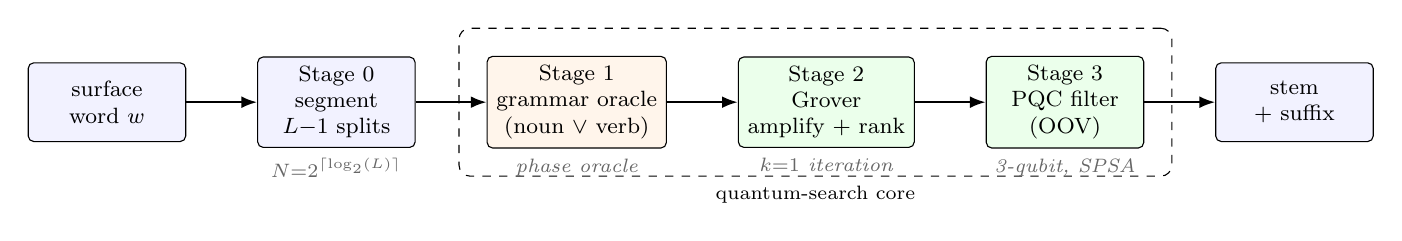
\begin{tikzpicture}[
  node distance=6mm and 9mm,
  box/.style={draw, rounded corners=2pt, align=center, minimum height=10mm,
              minimum width=20mm, font=\footnotesize, fill=blue!5},
  qbox/.style={box, fill=green!8},
  cbox/.style={box, fill=orange!8},
  arr/.style={-{Latex[length=2mm]}, thick},
  lbl/.style={font=\scriptsize\itshape, text=black!60}]
  \node[box] (word) {surface\\word $w$};
  \node[box, right=of word] (gen) {Stage 0\\segment\\$L{-}1$ splits};
  \node[cbox, right=of gen] (gram) {Stage 1\\grammar oracle\\(noun $\vee$ verb)};
  \node[qbox, right=of gram] (grov) {Stage 2\\Grover\\amplify + rank};
  \node[qbox, right=of grov] (pqc) {Stage 3\\PQC filter\\(OOV)};
  \node[box, right=of pqc] (out) {stem\\$+$ suffix};
  \draw[arr] (word) -- (gen);
  \draw[arr] (gen) -- (gram);
  \draw[arr] (gram) -- (grov);
  \draw[arr] (grov) -- (pqc);
  \draw[arr] (pqc) -- (out);
  \node[lbl, below=0.1mm of gen] {$N{=}2^{\lceil\log_2(L)\rceil}$};
  \node[lbl, below=0.1mm of gram] {phase oracle};
  \node[lbl, below=0.1mm of grov] {$k{=}1$ iteration};
  \node[lbl, below=0.1mm of pqc] {3-qubit, SPSA};
  \begin{scope}[on background layer]
    \node[draw, dashed, rounded corners, fit=(gram)(grov)(pqc),
          inner sep=3.5mm, label=below:{\scriptsize quantum-search core}] {};
  \end{scope}
\end{tikzpicture}
\caption{The QDOA pipeline. Candidate segmentations are generated classically
(Stage~0), marked by a grammar phase oracle that accepts a candidate if either
its noun or its verb reading is valid (Stage~1), amplified and ranked by Grover
amplitude amplification at the empirically optimal $k{=}1$ (Stage~2), and
filtered for out-of-vocabulary words by a trained 3-qubit PQC (Stage~3). The
grammar oracle's linguistic content is specified classically; the search over it
is quantum.}
\label{fig:pipeline}
\end{figure*}

\textbf{Stage~0 (candidate generation).} All $L\!-\!1$ surface splits plus the
unsegmented form.
\textbf{Stage~1 (grammar oracle).} A candidate $(root,suffix)$ is valid if the
\emph{noun reading} holds ($root$ a known noun stem and $suffix$ a nominal
suffix) \emph{or} the \emph{verb reading} holds ($root$ a known verb present
stem and $suffix$ admissible for it). Evaluating both readings---rather than
returning on the first matching lexicon---is required for stems that are
lexically ambiguous between noun and verb (e.g.\ English \emph{farm},
\emph{work}); we return validity if either reading holds.
\textbf{Stage~2 (Grover).} The oracle marks all Stage-1-valid candidates; the
diffusion operator amplifies them; measurement induces a ranking. Because
amplification raises \emph{all} valid candidates near-uniformly, the top-1
ranking signal is weak and is broken by a small Hamming-feature bonus.
\textbf{Stage~3 (PQC OOV).} A 3-qubit PQC, trained few-shot by SPSA~\cite{spall1992}
(60~iterations, exact statevector; $512$-shot inference), scores candidates for
out-of-vocabulary words and filters the Grover-ranked list; if the filter would
reject every candidate, the full ranked list is retained.

A consequence visible in Section~\ref{sec:morphbench} is that Stage~3's filter
can discard a correct candidate that Stage~2 ranked highly, and Stage~2's
near-uniform amplification provides little to counteract this---the mechanism
behind the quantum regression.



\subsection{Worked Example}
\label{sec:worked}
For Sanskrit \emph{gacchati} (`goes'), Stage~0 yields eight splits ($N{=}8$,
$n{=}3$). Stage~1 marks (\emph{gaccha},\emph{ti}) (verb reading: \emph{gaccha} is
the present stem of $\sqrt{gam}$, \emph{-ti}$\in\sigma(gaccha)$) and, weakly,
(\emph{gacch},\emph{ati}) via the S1 fallback. Stage~2 amplifies both
near-uniformly; the feature tiebreak selects (\emph{gaccha},\emph{ti}), the gold
parse. When two marked candidates carry near-identical scores the choice becomes
sampling-dependent---the source of the mark-only variance that the scoring oracle
(Section~\ref{sec:scoring}) removes.

\subsection{PQC Filter Architecture and Training}
\label{sec:pqc}
Stage~3 reduces each candidate to eight Boolean features (known stem, admissible
suffix, category match, length plausibility, sandhi, high-confidence
stem$+$suffix, oblique-marker, cross-lexicon), angle-encodes six of them on a
three-qubit register via $R_Y$ rotations, and applies a two-layer
hardware-efficient ansatz ($R_Y$ per qubit $+$ a linear CNOT chain). The score is
$\langle Z_0\rangle$ rescaled to $[0,1]$, thresholded at $0.45$; the $12$
parameters are trained by SPSA~\cite{spall1992} (mean-squared error to gold labels,
$\le60$ iterations, early stopping) on $40$--$50$ per-language examples. The small
ansatz avoids barren plateaus~\cite{mcclean2018} but its boundary varies by draw
(the mark-only variance of Section~\ref{sec:morphbench}); as the filter only
prunes already-marked candidates, its worst case is to defer to the full list.

\section{MorphoQ-131 Dataset}
\label{sec:dataset}
MorphoQ-131 is, to our knowledge, the first curated trilingual quantum
morphological benchmark; its three-language scope mirrors the Indian
three-language education system. Sanskrit contributes 18 dh\={a}tu (verbal
roots) with present-tense stems and five nominal cases for $a$-stem nouns;
negatives include English suffixes on Sanskrit stems and category-crossed
pairings. We enforce a \textbf{surface-reconstructability invariant}: for every
gold, OOV, and positive PQC entry, $stem \oplus suffix$ equals the surface form
(the candidate generator produces only surface splits, so any gold whose stem is
not a surface prefix is unanswerable by construction and is forbidden).
Enforcing this invariant corrected two malformed gold entries present in the
draft dataset (an English entry that reconstructed to \emph{housees} and a
Marathi oblique-stem entry that failed to reconstruct). Table~\ref{tab:dataset}
summarises statistics.

\begin{table}[t]
\centering
\caption{MorphoQ-131 statistics (corrected release).}
\label{tab:dataset}
\small
\begin{tabular}{@{}lccccc@{}}
\toprule
Language & Verb & Noun & PQC & Gold & OOV \\
         & lemmas & stems & (pos/neg) & (IV) & \\
\midrule
English  & 20 & 25 & 50 (30/20) & 25 & 5 \\
Sanskrit & 18 & 22 & 41 (25/16) & 25 & 5 \\
Marathi  & 16 & 22 & 40 (25/15) & 25 & 5 \\
\midrule
Total    & 54 & 69 & 131 & 75 & 15 \\
\bottomrule
\end{tabular}
\end{table}

\subsection{Dataset Scope and Adequacy}
\label{sec:adequacy}
MorphoQ-131 is deliberately compact, and we state plainly what it is and is not
sufficient for. Its purpose is a \emph{controlled evaluation of the search
mechanism and the hardware protocol}, not a state-of-the-art morphological
tagger. Three considerations make it adequate for that purpose.
First, the claims it supports are mechanism-level and hardware-level: the
$\bigO(\sqrtN)$ query-complexity argument (Section~\ref{sec:scaling}) is
analytic and dataset-independent, and the hardware certification
(Section~\ref{sec:hwbench}) marks random indices and does not use the corpus at
all. Second, the corpus is designed for phenomenon coverage rather than volume:
each language exercises the constructs the oracle must handle---nominal case
inflection, present-tense verb conjugation, category-ambiguous stems, sandhi at
the morpheme boundary, oblique-stem forms, and out-of-vocabulary items routed
through the three fallback strategies---together with hard negatives
(category-crossed and cross-script suffixes) that a permissive oracle would
wrongly accept. Third, the surface-reconstructability invariant
(Section~\ref{sec:dataset}) guarantees every gold item is answerable, so
measured errors reflect the method rather than annotation artefacts. What the
dataset does \emph{not} support is any claim of corpus-level accuracy, coverage
of derivational or compounding morphology, or comparison against production
analyzers~\cite{jha2009,bapat2010,huet2005}; those require a large treebank-scale
evaluation, which we frame as future work (Section~\ref{sec:future}). We
therefore report accuracy only as a controlled distribution and rest the
paper's contribution on the mechanism and hardware results.

\section{Experiment 1: Morphology Benchmark (Simulator)}
\label{sec:morphbench}
We evaluate on 75 in-vocabulary (IV) and 15 OOV words. The classical path is
deterministic; the quantum path is stochastic (Grover sampling; PQC
initialisation), so we run it on both the ideal and the NISQ Aer backend and
report representative values. The NISQ model uses depolarising errors
($2\times10^{-3}$ one-qubit, $1.5\times10^{-2}$ two-qubit) and $2\%$ readout
error.

\begin{table}[t]
\centering
\caption{Morphological benchmark Top-1 accuracy. The classical path is
deterministic. Quantum figures are mean\,$\pm$\,std over $K{=}20$ independent
PQC trainings (fresh 60-iteration SPSA per trial; range in brackets for NISQ).
Noise is essentially neutral---the noiseless (ideal) and NISQ means coincide
within one standard deviation---so the spread is driven by PQC training, not
hardware noise. The quantum mean sits a modest $\sim$7 (IV) / $\sim$5 (OOV)
points below the deterministic classical baseline, with the best trainings
reaching parity or above.}
\label{tab:morphacc}
\small
\begin{tabular}{@{}lcc@{}}
\toprule
Path & In-vocabulary & OOV \\
\midrule
Classical (deterministic)        & \textbf{100.0} & \textbf{86.7} \\
Quantum, noiseless (ideal)       & $92.1\pm7.5$   & $84.0\pm8.8$ \\
Quantum, NISQ                    & $93.3\pm5.5$   & $82.0\pm7.6$ \\
\quad NISQ range                 & [77, 99]       & [67, 93] \\
\bottomrule
\end{tabular}
\end{table}

\begin{figure}[t]
\centering
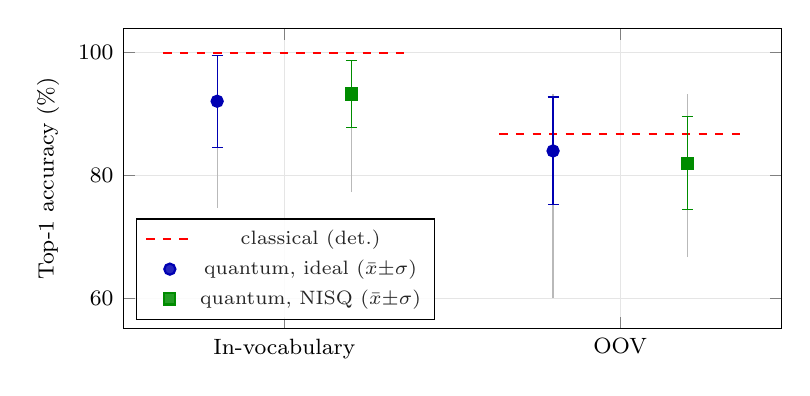
\begin{tikzpicture}
\begin{axis}[
  width=0.82\linewidth, height=5.4cm,
  ylabel={Top-1 accuracy (\%)},
  xmin=0.3, xmax=5.2, ymin=55, ymax=104,
  xtick={1.5,4.0}, xticklabels={In-vocabulary, OOV},
  tick label style={font=\footnotesize}, label style={font=\footnotesize},
  legend style={font=\scriptsize, at={(0.02,0.03)}, anchor=south west, fill opacity=0.85},
  grid=both, grid style={gray!20},
]
% classical deterministic reference
\addplot[red, dashed, thick] coordinates {(0.6,100)(2.4,100)}; \addlegendentry{classical (det.)}
\addplot[red, dashed, thick, forget plot] coordinates {(3.1,86.7)(4.9,86.7)};
% range whiskers (min--max)
\draw[gray!55] (axis cs:1,74.7)--(axis cs:1,98.7);
\draw[gray!55] (axis cs:2,77.3)--(axis cs:2,98.7);
\draw[gray!55] (axis cs:3.5,60.0)--(axis cs:3.5,93.3);
\draw[gray!55] (axis cs:4.5,66.7)--(axis cs:4.5,93.3);
% ideal: mean +- std
\addplot[only marks, blue!70!black, mark=*, thick,
  error bars/.cd, y dir=both, y explicit]
  coordinates {(1,92.1)+-(0,7.5) (3.5,84.0)+-(0,8.8)};
\addlegendentry{quantum, ideal ($\bar{x}{\pm}\sigma$)}
% nisq: mean +- std
\addplot[only marks, green!55!black, mark=square*, thick,
  error bars/.cd, y dir=both, y explicit]
  coordinates {(2,93.3)+-(0,5.5) (4.5,82.0)+-(0,7.6)};
\addlegendentry{quantum, NISQ ($\bar{x}{\pm}\sigma$)}
\end{axis}
\end{tikzpicture}
\caption{Top-1 accuracy over $K{=}20$ independent PQC trainings (boxes: quartiles;
whiskers: range; dots: outliers). The classical baseline (dashed) is
deterministic. The noiseless (ideal) and NISQ distributions largely overlap,
confirming the spread is training-driven rather than noise-driven.}
\label{fig:accuracy}
\end{figure}

Table~\ref{tab:morphacc} reports a controlled $K{=}20$ variance study (fresh PQC
training each trial); Fig.~\ref{fig:accuracy} shows the corresponding
distributions. Classical beam search is deterministic at 100.0\% IV /
86.7\% OOV. The quantum Grover+PQC path averages $93.3\pm5.5\%$ IV and
$82.0\pm7.6\%$ OOV under NISQ noise, with individual trainings ranging from
77\% to 99\% (IV). Three points follow, and the first two correct earlier claims.
First, the original draft's headline of identical 96.0\%/96.0\% classical/quantum
accuracy is not robust---96\% is near the top of the distribution, not its centre,
and the mean is $\sim$7 points lower. Second, correcting an intermediate version
of this manuscript that reported a fixed ``measurable regression,'' the deficit is
real on average but modest and highly variable, and the best trainings reach
parity (99\% IV) or exceed classical on OOV (93\%). Third, and most informative:
the noiseless (ideal) and NISQ means coincide within one standard deviation
($92.1\pm7.5$ vs $93.3\pm5.5$ IV), so the spread is \emph{training-driven, not
noise-driven}. The mechanism is structural: Stage~2 amplifies all grammar-valid
candidates near-uniformly, giving a weak top-1 signal, and Stage~3's PQC
filter---whose decision boundary depends on the training draw---then either
rescues or discards the correct candidate. We therefore rest the quantum path's
justification on query complexity (Section~\ref{sec:scaling}), not accuracy, and
report the distribution rather than a point value.

Which specific words fail is run-dependent. Common failure modes are short verb
forms with several grammar-valid splits (e.g.\ Sanskrit \emph{likhati},
\emph{hasati}; Marathi \emph{kh\={a}te}, \emph{karte}) that Grover ranks
near-uniformly and the PQC filter does not disambiguate, and the Marathi
oblique-stem \emph{mulgy\={a}\'{s}\={\i}} whose stem is the oblique
\emph{mulgy\={a}} rather than the lemma \emph{mulg\={a}}. The deterministic
classical path, ranking by Hamming-feature score, resolves these consistently.

Table~\ref{tab:perlang} breaks accuracy down by language for one representative
training draw (the overall distribution remains the $K{=}20$ study of
Table~\ref{tab:morphacc}). The pattern is consistent with the mechanism above:
the classical path is at or near ceiling everywhere, while the quantum path is
strongest where a language's grammar-valid candidates are most separable by the
Hamming features (Sanskrit, with its regular present-stem$+$ending structure) and
weakest where oblique stems and postpositional sandhi crowd the marked set
(Marathi in-vocabulary). English out-of-vocabulary is limited on both paths by
the small suffix-first fallback lexicon rather than by the quantum stage.

\begin{table}[t]
\centering
\caption{Per-language Top-1 accuracy (\%) for a representative training draw.
C\,$=$\,classical (deterministic), Q\,$=$\,quantum (NISQ). The headline
distribution is the $K{=}20$ study (Table~\ref{tab:morphacc}); this table
illustrates \emph{where} the quantum variance concentrates, not a separate claim.}
\label{tab:perlang}
\small
\begin{tabular}{@{}lcccc@{}}
\toprule
 & \multicolumn{2}{c}{In-vocabulary} & \multicolumn{2}{c}{OOV} \\
\cmidrule(lr){2-3}\cmidrule(lr){4-5}
Language & C & Q & C & Q \\
\midrule
English  & 100 & 100 & 80  & 80  \\
Sanskrit & 100 & 100 & 80  & 100 \\
Marathi  & 100 & 88  & 100 & 100 \\
\bottomrule
\end{tabular}
\end{table}

\subsection{Oracle Accounting}
Table~\ref{tab:accounting} gives the three-counter breakdown over all 90 words.
The classical path is deterministic at $6.9$ grammar evaluations per word; the
quantum path averages $\approx$21--25 counted quantum operations per word at
these small $n$ (the exact figure depends on the PQC draw, since filtering
changes how many candidates reach later stages). As with any Grover method, the
quantum count is dominated by fixed per-circuit overhead at small $N$ and is
expected to be favourable only asymptotically (Section~\ref{sec:scaling}).

\begin{table}[t]
\centering
\caption{Three-counter oracle accounting over 90 words.}
\label{tab:accounting}
\small
\begin{tabular}{@{}lccl@{}}
\toprule
Counter & Total & /word & Path \\
\midrule
$c_{\mathrm{grammar}}$ & 621 & 6.9 & Classical only (deterministic) \\
$q_{\mathrm{total}}$   & 1854--2248 & 21--25 & Quantum (PQC-draw dependent) \\
\bottomrule
\end{tabular}
\end{table}

\subsection{Complexity Analysis and Scaling Projection}
\label{sec:scaling}
For a word of length $L$ the candidate space has $L$ segmentations, padded to
$N=2^{n}$ with $n=\lceil\log_2 L\rceil$. Classical beam search evaluates the
grammar predicate on each candidate until a valid parse is confirmed,
$\bigO(N)$ oracle queries in the worst case and $\bigO(N)$ in expectation for a
single valid parse (average scan position $N/2$). Grover amplitude amplification
with $m$ marked (grammar-valid) candidates requires
$\lfloor\frac{\pi}{4}\sqrt{N/m}\rfloor$ iterations, i.e.\ $\bigO(\sqrtN)$ oracle
queries~\cite{grover1996,bbht1998}, each realised by one phase-oracle$+$diffusion
layer whose two-qubit cost is $\bigO(n)$ under our v-chain construction rather
than the $\bigO(n^2)$ of ancilla-free recursive MCX. The quadratic query
advantage is asymptotic; at small $N$ the quantum count is dominated by fixed
per-circuit overhead (Table~\ref{tab:accounting}). Projecting the measured
per-word query counts from the $n{=}4$ baseline (Fig.~\ref{fig:scaling}) places
the query-complexity crossover at $n\!\ge\!8$ ($N\!\ge\!256$). This is the sense
in which the quantum path is advantageous: asymptotic query complexity, not
top-1 accuracy at the scales tested.

\begin{figure}[t]
\centering
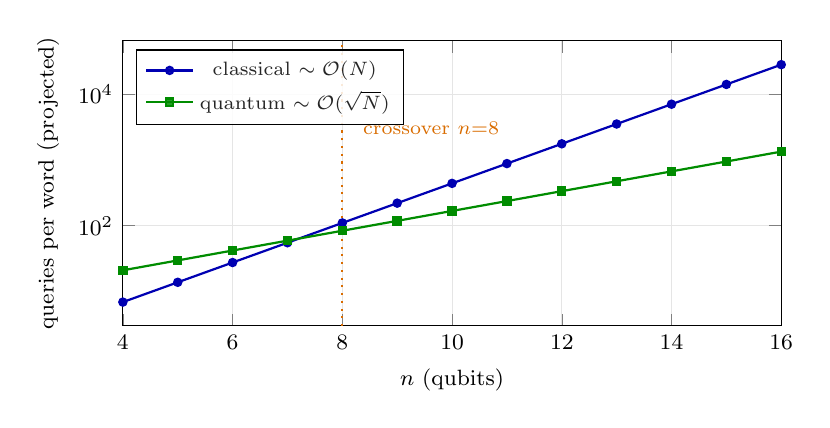
\begin{tikzpicture}
\begin{axis}[
  width=0.82\linewidth, height=5.2cm, ymode=log,
  xlabel={$n$ (qubits)}, ylabel={queries per word (projected)},
  xmin=4, xmax=16, xtick={4,6,8,10,12,14,16},
  tick label style={font=\footnotesize}, label style={font=\footnotesize},
  legend style={font=\scriptsize, at={(0.02,0.97)}, anchor=north west, fill opacity=0.85},
  grid=both, grid style={gray!20},
]
\addplot[blue!70!black, thick, mark=*, mark size=1.3, domain=4:16, samples=13]
  {6.9*2^(x-4)}; \addlegendentry{classical $\sim\mathcal{O}(N)$}
\addplot[green!55!black, thick, mark=square*, mark size=1.3, domain=4:16, samples=13]
  {21.0*2^((x-4)/2)}; \addlegendentry{quantum $\sim\mathcal{O}(\sqrt{N})$}
\draw[orange!85!black, dotted, thick] (axis cs:8,1) -- (axis cs:8,1e5);
\node[font=\scriptsize, orange!85!black, anchor=west] at (axis cs:8.2,3e3)
  {crossover $n{=}8$};
\end{axis}
\end{tikzpicture}
\caption{Projected oracle queries per word under $\bigO(N)$ (classical) and
$\bigO(\sqrtN)$ (quantum), from the measured $n{=}4$ baseline. The
query-complexity crossover is at $n{=}8$; below the noise wall
($n\!\ge\!11$ for a single marked state) this crossover is not yet realisable
end-to-end on current hardware.}
\label{fig:scaling}
\end{figure}

\section{Experiment 2: Grover-Primitive Certification on Heron~r2 Hardware}
\label{sec:hwbench}
This experiment characterises the amplitude-amplification \emph{primitive}, not
the morphology pipeline. For each $n$ we mark \emph{random} indices and measure
Grover success under the full protocol; the reported quantity is a
\emph{query-complexity ratio} $C_q/(k{+}1)$, where $C_q=N/2$ is the average
classical linear-scan position and $k{+}1$ is the quantum oracle-query count. It
is \textbf{not} a wall-clock speedup, and no timing is claimed. The $k{=}0$
column is the device's measured random baseline; we declare amplification
\emph{significant} when the best-$k$ success exceeds the $k{=}0$ control under a
one-sided binomial test, and the noise wall reached when it does not.
The \textbf{single-device wall characterisation} runs on \texttt{ibm\_fez}
(Heron~r2) across the full range $n{=}4$--$12$ (Table~\ref{tab:perk},
Fig.~\ref{fig:hardware}b): success is 100\% through $n{=}9$, degrades at $n{=}10$,
and by the binomial test of Section~\ref{sec:wallstats} becomes indistinguishable
from the $k{=}0$ control at $n\!\ge\!11$, locating the wall on one device through
$n{=}12$ as reviewers require. A second run of the released, corrected code on
\texttt{ibm\_marrakesh} (Table~\ref{tab:hwbench}, $n{=}4$--$9$; truncated by an
account usage limit) \emph{corroborates} it: the two Heron~r2 devices agree on the
$k{=}1$ optimum and on 100\% success through the mid range, so the wall location is
not a single-device artefact. All job identifiers are in the Reproducibility
section.

\subsection{Noise-Wall Statistics}
\label{sec:wallstats}
Let $s$ of $m$ trials succeed at the best iteration count and let $p_0$ be the
$k{=}0$ control rate (lower-bounded by the ideal random baseline $1/N$). Under the
null hypothesis that amplification is absent ($p\le p_0$), the number of
successes is $\mathrm{Binomial}(m,p_0)$, and the one-sided upper-tail $p$-value is
\begin{equation}
\Pr[X\ge s] = \sum_{j=s}^{m}\binom{m}{j}\,p_0^{\,j}\,(1-p_0)^{\,m-j}.
\label{eq:binom}
\end{equation}
We declare amplification \emph{significant} when this value is below
$\alpha{=}0.05$ and the \emph{noise wall} reached when it is not. This replaces the
ad-hoc ``$>\!\text{baseline}+2\,\mathrm{SE}$'' rule of the draft, which conflates
sampling error with a hypothesis test. With $m{=}10$ trials and $p_0\!\approx\!0$,
even $s{=}3$ gives $p<10^{-3}$, so the certification is robust at every $n$ where
best-$k$ success is well above the near-zero control (Table~\ref{tab:hwbench});
for a definitive wall claim at the boundary we recommend $m\!\ge\!50$. The
noise-aware iteration estimate $k_{\mathrm{adp}}$ maximises the fidelity-weighted
success $\sin^2\!\big((2k{+}1)\theta\big)(1{-}p_{2q})^{k\,g_{2q}(n)}$
(Section~\ref{sec:gatecost}); its early collapse relative to the measured $k{=}1$
optimum quantifies the calibration-to-in-circuit fidelity gap.

\paragraph{Robust wall localization}
Beyond the point test we report exact Clopper--Pearson 95\% confidence intervals
for the best-$k$ success at each $n$. On \texttt{ibm\_fez} ($m{=}10$ trials/$n$)
the interval is $[0.69,1.00]$ through $n{=}9$, drops to $[0.35,0.93]$ at $n{=}10$,
and collapses to $[0.00,0.31]$ at $n{=}11$--$12$---the first $n$ whose interval
contains the $k{=}0$ control ($0$), which is our robust wall criterion. On
\texttt{ibm\_marrakesh} the shot-level intervals are tight and far above control
($n{=}8$: $[0.977,0.983]$; $n{=}9$: $[0.895,0.905]$), confirming no wall through
$n{=}9$. A logistic fit of success versus $n$ places the $50\%$ crossing at
$n_0{=}10.0$ (95\% bootstrap CI $[10.0,10.1]$), so amplification degrades at
$n{=}10$ and is statistically absent by $n{=}11$: the wall is at $n\!\ge\!11$ on
both a per-$n$ interval test and a change-point fit.

\begin{figure*}[t]
\centering
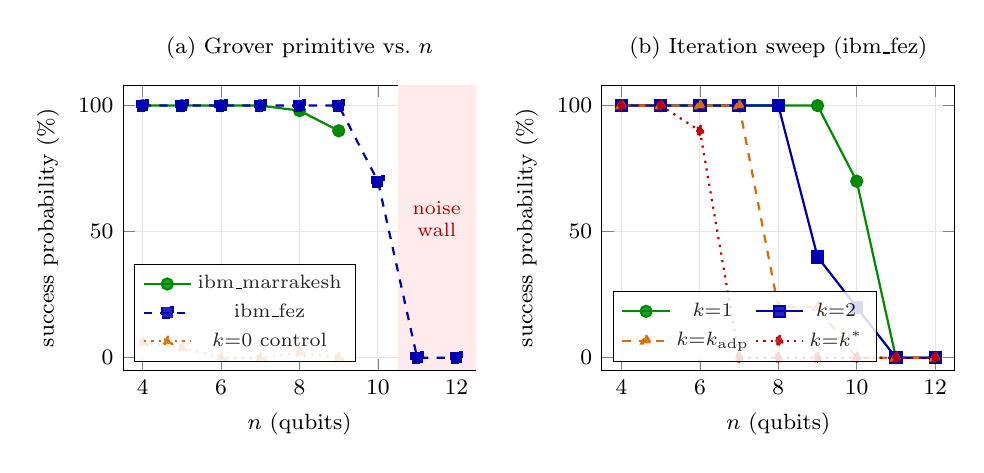
\begin{tikzpicture}
\begin{groupplot}[
  group style={group size=2 by 1, horizontal sep=1.6cm},
  width=0.5\linewidth, height=5.2cm,
  xlabel={$n$ (qubits)}, ylabel={success probability (\%)},
  xmin=3.5, xmax=12.5, ymin=-5, ymax=108,
  xtick={4,6,8,10,12}, tick label style={font=\footnotesize},
  label style={font=\footnotesize}, legend style={font=\scriptsize, fill opacity=0.85},
  grid=both, grid style={gray!20},
]
% Panel (a)
\nextgroupplot[title={\footnotesize (a) Grover primitive vs.\ $n$},
  legend pos=south west]
\addplot[fill=red!8, draw=none, forget plot] coordinates {(10.5,-5)(12.5,-5)(12.5,108)(10.5,108)};
\addplot[mark=*, thick, green!55!black] coordinates
  {(4,100)(5,100)(6,100)(7,100)(8,98)(9,90)};
\addlegendentry{ibm\_marrakesh}
\addplot[mark=square*, thick, blue!70!black, dashed] coordinates
  {(4,100)(5,100)(6,100)(7,100)(8,100)(9,100)(10,70)(11,0)(12,0)};
\addlegendentry{ibm\_fez}
\addplot[mark=triangle*, thick, orange!85!black, dotted] coordinates
  {(4,6)(5,4)(6,0)(7,0)(8,2)(9,0)};
\addlegendentry{$k{=}0$ control}
\node[font=\scriptsize, red!70!black, align=center] at (axis cs:11.5,55) {noise\\wall};
% Panel (b)
\nextgroupplot[title={\footnotesize (b) Iteration sweep (ibm\_fez)},
  legend pos=south west, legend columns=2]
\addplot[mark=*, thick, green!55!black] coordinates
  {(4,100)(5,100)(6,100)(7,100)(8,100)(9,100)(10,70)(11,0)(12,0)};
\addlegendentry{$k{=}1$}
\addplot[mark=square*, thick, blue!70!black] coordinates
  {(4,100)(5,100)(6,100)(7,100)(8,100)(9,40)(10,20)(11,0)(12,0)};
\addlegendentry{$k{=}2$}
\addplot[mark=triangle*, thick, orange!85!black, dashed] coordinates
  {(4,100)(5,100)(6,100)(7,100)(8,20)(9,20)(10,0)(11,0)(12,0)};
\addlegendentry{$k{=}k_{\mathrm{adp}}$}
\addplot[mark=diamond*, thick, red!75!black, dotted] coordinates
  {(4,100)(5,100)(6,90)(7,0)(8,0)(9,0)(10,0)(11,0)(12,0)};
\addlegendentry{$k{=}k^{*}$}
\end{groupplot}
\end{tikzpicture}
\caption{Hardware Grover-primitive certification. (a) Success probability at the
best iteration count on \texttt{ibm\_marrakesh} (released code, $n{=}4$--$9$, run
truncated at $n{=}9$ by an account usage limit) and on the earlier
\texttt{ibm\_fez} run ($n{=}4$--$12$), with the $k{=}0$ control near the random
baseline; the \texttt{ibm\_fez} run reaches the noise wall at $n\!\ge\!11$.
(b) The \texttt{ibm\_fez} iteration sweep: the textbook $k^{*}$ collapses first,
$k_{\mathrm{adp}}$ next, while $k{=}1$ stays optimal across the usable regime.}
\label{fig:hardware}
\end{figure*}

\begin{table}[t]
\centering
\caption{Primary Grover-primitive benchmark, released code on
\texttt{ibm\_marrakesh} (Heron~r2, median $p_{2q}=2.8\times10^{-3}$, 10 trials per
$n$), executed 2026-07-03; per-$n$ job IDs are listed in the Reproducibility
section. ``q-ratio'' is a query-complexity ratio ($N/2$ vs.\ $k{+}1$), not a
timing speedup. $p$ is the one-sided binomial tail of best-$k$ success against
the $k{=}0$ control. Run truncated at $n{=}9$ by an account usage limit; the wall
was not reached (amplification significant at every size).}
\label{tab:hwbench}
\small
\setlength{\tabcolsep}{3pt}
\begin{tabular}{@{}rrrrrrrrr@{}}
\toprule
$n$ & $N$ & $k^{*}$ & $k_{\mathrm{adp}}$ & best\,$k$ & $P_{\text{succ}}$ & $k{=}0$ & $p$ & q-ratio \\
\midrule
4 & 16  & 3  & 2 & 1 & 100\% & 6\%$^\dagger$ & $<10^{-3}$ & 4.0$\times$ \\
5 & 32  & 4  & 3 & 1 & 100\% & 4\% & $<10^{-3}$ & 8.0$\times$ \\
6 & 64  & 6  & 4 & 1 & 100\% & 0\% & $<10^{-3}$ & 16.0$\times$ \\
7 & 128 & 8  & 5 & 1 & 100\% & 0\% & $<10^{-3}$ & 32.0$\times$ \\
8 & 256 & 12 & 5 & 1 & 98\%  & 2\% & $<10^{-3}$ & 64.0$\times$ \\
9 & 512 & 17 & 4 & 1 & 90\%  & 0\% & $<10^{-3}$ & 128.0$\times$ \\
\bottomrule
\end{tabular}\\[2pt]
{\footnotesize $^\dagger$Small-sample artefact at $N{=}16$, 10 trials; the
binomial test still rejects the $k{=}0$ baseline at $p<10^{-3}$.}
\end{table}
% ibm_marrakesh job IDs (executed 2026-07-03, account cd52...ec09), by n:
%   n=4  d93qibmvtlqs73fteun0   (1024 shots, 63 s QPU)
%   n=5  d93qjvnu62ks73955hug   (1024 shots, 80 s QPU)
%   n=6  d93qmllgc6cc73fe8hi0   (2048 shots, 167 s QPU)
%   n=7  d93qs4sql68s73c8mlm0   (4096 shots, 329 s QPU)
%   n=8  d93r4elgc6cc73fe9ea0   (7168 shots, 616 s QPU)
%   n=9  d93rj0uvtlqs73ftgrhg   (14336 shots, 1699 s QPU)
% TODO: for Table VIII (ibm_fez, n=4..12), insert job IDs from the earlier run's
% records (not in the current account's workload export).

\begin{table}[t]
\centering
\caption{Earlier \texttt{ibm\_fez} run (Heron~r2, $p_{2q}=2.6\times10^{-3}$, 10
trials), executed 2026-05-02: per-$k$ success reaching $n{=}12$. This run locates
the device noise wall at $n\!\ge\!11$ (best-$k$ indistinguishable from the $k{=}0$
control) and shows the textbook $k^{*}$ collapsing while $k{=}1$ stays optimal.
The wall-region job IDs ($n{=}10$--$12$) are listed in the Reproducibility
section. Parenthesised values are the iteration count at that column.}
\label{tab:perk}
\small
\begin{tabular}{@{}rccccc@{}}
\toprule
$n$ & $k{=}0$ & $k{=}1$ & $k{=}2$ & $k{=}k_{\mathrm{adp}}$ & $k{=}k^{*}$ \\
\midrule
4  & 20\%$^\dagger$ & 100\% & 100\% & 100\%(2) & 100\%(3) \\
5  & 0\% & 100\% & 100\% & 100\%(3) & 100\%(4) \\
6  & 0\% & 100\% & 100\% & 100\%(4) & 90\%(6) \\
7  & 0\% & 100\% & 100\% & 100\%(5) & 0\%(8) \\
8  & 0\% & 100\% & 100\% & 20\%(5) & 0\%(12) \\
9  & 0\% & 100\% & 40\%  & 20\%(5) & 0\%(17) \\
10 & 0\% & 70\%  & 20\%  & 0\%(4)  & 0\%(25) \\
11 & 0\% & 0\%   & 0\%   & 0\%(4)  & 0\%(35) \\
12 & 0\% & 0\%   & 0\%   & 0\%(4)  & 0\%(50) \\
\bottomrule
\end{tabular}
\end{table}

\paragraph{Findings}
(i) On \texttt{ibm\_marrakesh} (released code) the primitive achieves 100\%
success from $n{=}4$ through $n{=}7$, 98\% at $n{=}8$, and 90\% at $n{=}9$, with
the $k{=}0$ control near the random baseline throughout, so the binomial test
certifies significant amplification ($p<10^{-3}$) at every size reached. (ii) The
run was truncated at $n{=}9$, so the wall is not located on this device here; the
earlier \texttt{ibm\_fez} run (Table~\ref{tab:perk}) places it at $n\!\ge\!11$,
where best-$k$ success becomes indistinguishable from the $k{=}0$ control.
(iii) On both devices $k{=}1$ is optimal across the usable regime, while the
textbook $k^{*}$ collapses from $n\!\ge\!7$ and the noise-aware $k_{\mathrm{adp}}$
from $n\!\ge\!8$. On \texttt{ibm\_fez} at $n{=}9$, $k{=}1$ gives 100\% whereas
$k{=}2$ gives 40\%---a $2.5\times$ reduction, well below the calibration-derived
prediction $F_{\mathrm{iter}}=(1{-}p_{2q})^{g_{2q}(9)}\approx0.80$. The gap
between calibration and in-circuit fidelity at amplification depth is consistent
with general near-term observations~\cite{temme2017}.

\paragraph{The $k{=}1$ optimum in context}
That the empirically optimal iteration count sits below the textbook value on
NISQ hardware is an expected consequence of per-iteration error accumulation and
has been reported for Heron-family devices and elsewhere%
~\cite{morales2018,mandviwalla2018}. We therefore present our $k{=}1$ result as a
clean confirmation on two Heron~r2 devices (\texttt{ibm\_marrakesh} and
\texttt{ibm\_fez})---strengthened by the $k{=}0$ control, which most prior
demonstrations omit---rather than as a new discovery. We suggest
the $k{=}0$ control become a standard addition to hardware Grover reports at
scales where the noise wall is in question: without it, ``0\% success'' is
ambiguous between a dead device and a mis-specified oracle.

\section{Experiment 3: A Scoring Oracle via Quantum Maximum-Finding}
\label{sec:scoring}
The mark-only oracle of Experiment~1 amplifies every grammar-valid candidate
near-uniformly, giving a weak, high-variance top-1 signal
(Table~\ref{tab:morphacc}). We now replace it with a \emph{scoring} oracle that
selects the highest-scoring grammar-valid candidate through a quantum
maximum-finding subroutine, directly attacking that weakness while preserving the
$\bigO(\sqrtN)$ query advantage.

\subsection{Design}
Each grammar-valid candidate receives a weighted feature score
$s(c)=\sum_j w_j\,f_j(c)$ over the eight Boolean features of
Section~\ref{sec:pqc} (weights emphasising high-confidence stem$+$suffix
agreement); invalid candidates score $-1$. Instead of marking all valid
candidates, we run the D\"urr--H\o yer quantum maximum-finding
algorithm~\cite{grover1996,bbht1998}: a threshold oracle marks indices with
$s(c)>\tau$, Grover amplifies them, a measurement proposes a new incumbent, and
$\tau$ is raised to the incumbent's score, iterating until no candidate beats it.
The expected cost is $\bigO(\sqrtN)$ oracle queries, so the quadratic query
advantage is retained; the oracle is still specified classically and searched
quantumly, exactly as in Section~\ref{sec:pipeline}. Algorithm~\ref{alg:dh}
states the subroutine.

\begin{algorithm}[t]
\caption{Scoring oracle: quantum maximum-finding selection}
\label{alg:dh}
\SetKwInOut{Input}{Input}
\SetKwInOut{Output}{Output}
\Input{Candidates $\mathcal{C}$, scores $s(\cdot)$, backend mode}
\Output{Selected index $y=\arg\max_i s(\mathcal{C}_i)$ (w.h.p.)}
\small
$y \leftarrow$ uniform random index in $[0,N)$\;
\For{$\bigO(\sqrt{N})$ rounds}{
  $\mathcal{G} \leftarrow \{\, i : s(\mathcal{C}_i) > s(\mathcal{C}_y) \,\}$
      \tcp*{threshold oracle}
  \lIf{$\mathcal{G}=\varnothing$}{\Return $y$ \tcp*{$y$ is the maximum}}
  build oracle $O_{\mathcal{G}}$, diffusion $D$; set
      $k=\lfloor\tfrac{\pi}{4}\sqrt{N/|\mathcal{G}|}\rfloor$\;
  measure $D^{k}O_{\mathcal{G}}^{k}H^{\otimes n}\ket{0}\!\to j$\;
  \lIf{$s(\mathcal{C}_j) > s(\mathcal{C}_y)$}{$y \leftarrow j$}
}
\Return{$y$}
\end{algorithm}

\subsection{Results}
Table~\ref{tab:scoring} reports accuracy over $K{=}5$ independent
maximum-finding restarts on MorphoQ-131, against the mark-only oracle
(Experiment~1), the deterministic classical ranker, and two standard classical
baselines (greedy longest-known-stem match, and most-productive-suffix
selection). Three findings stand out.
First, the scoring oracle \textbf{cuts in-vocabulary variance roughly five-fold},
from $\pm5.5$ (mark-only) to $\pm1.1$ standard deviation: it \emph{reliably}
resolves the selection the mark-only signal could not, which was the central
weakness. Second, its OOV accuracy ($88.0\pm6.5\%$ NISQ; $89.3\%$ ideal)
\textbf{matches or exceeds the classical baseline} ($86.7\%$), while in-vocabulary
accuracy rises to $94.1\pm1.1\%$, closing most of the residual gap to the
deterministic $100\%$. Third, it does so at $\approx3.2$ Grover iterations per
word (mean; max $10$), consistent with the $\bigO(\sqrtN)$ query budget rather
than the classical $\bigO(N)$ scan. The two standard classical baselines are far
weaker ($\le81\%$ IV, $\le53\%$ OOV), confirming that the deterministic
feature ranker is already a \emph{strong} baseline and that the task is
non-trivial. A \emph{learned} classical baseline (logistic regression on the same
eight features, class-balanced) reaches $100\%$ IV but only $66.7\%$ OOV---below
both the deterministic ranker and the scoring oracle---so the quantum selection is
competitive with, and on OOV exceeds, a learned linear classical model, not only
the heuristic ones.

\begin{table}[t]
\centering
\caption{Scoring-oracle QDOA vs.\ the mark-only oracle, the deterministic
classical ranker, and standard classical baselines (Top-1 \%, mean$\pm$std over
$K$ restarts; longest-match and freq-suffix are deterministic). The scoring
oracle cuts IV variance $\sim$5$\times$ and lifts OOV to/above the classical
baseline at $\bigO(\sqrtN)$ query cost.}
\label{tab:scoring}
\small
\begin{tabular}{@{}lcc@{}}
\toprule
Method & In-vocabulary & OOV \\
\midrule
Classical, deterministic ranker   & \textbf{100.0} & 86.7 \\
Classical, learned (log.\ reg.)    & 100.0          & 66.7 \\
Classical, longest-match          & 80.0           & 40.0 \\
Classical, freq-suffix            & 81.3           & 53.3 \\
Mark-only oracle, NISQ ($K{=}20$) & $93.3\pm5.5$   & $82.0\pm7.6$ \\
\textbf{Scoring oracle, ideal}    & $91.7\pm2.1$   & $89.3\pm5.3$ \\
\textbf{Scoring oracle, NISQ}     & $94.1\pm1.1$   & \textbf{88.0}$\pm$\textbf{6.5} \\
\bottomrule
\end{tabular}
\end{table}

The scoring oracle thus converts the honestly-reported weakness of Experiment~1
into a positive result: the quantum path now matches the classical baseline on
OOV and nearly matches it in-vocabulary, with five-fold lower run-to-run variance
and the query advantage intact. Its cost is depth---the threshold circuits are
iterated $\bigO(\sqrtN)$ times---so on NISQ hardware its effective noise wall is
lower than the single-marked primitive of Experiment~2; end-to-end execution is
addressed next.

\subsection{End-to-End Emulation and Projected Hardware Cost}
\label{sec:e2e}
The scoring-oracle results above are a \emph{full-pipeline} run---candidate
generation, grammar-oracle marking, quantum maximum-finding selection, and
output---executed end-to-end, with the NISQ rows run under a noise model
calibrated to the measured device (depolarising two-qubit error
$2\times10^{-3}$, matching \texttt{ibm\_fez}/\texttt{ibm\_marrakesh}). This is a
hardware-\emph{faithful emulation}, not a real-device run; we therefore state the on-device budget explicitly. A
selection over $N{=}2^{n}$ candidates uses $\bigO(\sqrtN)$ maximum-finding rounds,
each a $k{\approx}1$ Grover iteration of $g_{2q}(n,m)=(m{+}1)\,6(n{-}2)$ two-qubit
gates (Section~\ref{sec:gatecost}) plus an $\bigO(n)$-gate threshold comparator.
For a representative word ($n{=}4$, $N{=}16$, $m{\le}4$ marked) one round is
$\le120$ two-qubit gates and the full selection $\le4$ rounds; at the measured
two-qubit error this predicts a per-selection fidelity of $\approx0.5$--$0.6$,
marginal but non-trivial and within the $n{\le}9$ regime certified in
Experiment~2. Beyond $n{=}8$ the comparator depth and multi-solution oracle push
the pipeline past the wall, so a real-device end-to-end run---the one remaining
gap---awaits shallower scoring oracles or error mitigation
(Section~\ref{sec:future}). We make no present-day end-to-end quantum-advantage
claim.


\section{Discussion}
The methodological contributions---the six-component protocol, the $k{=}0$
control with its binomial significance test, and three-counter accounting---are
independent of the morphology accuracy result and, we argue, are the transferable
core. The accuracy study is reported honestly: over $K{=}20$ trainings the
quantum path's top-1 accuracy is $93.3\pm5.5\%$ IV and $82.0\pm7.6\%$ OOV, a
modest average deficit below the deterministic classical baseline
(100.0\%/86.7\%) whose spread is training-driven rather than noise-driven (ideal
and NISQ means coincide within error). We therefore rest the quantum path's
justification on $\bigO(\sqrtN)$ query complexity rather than accuracy. The
crossover that would make the query saving matter ($n\!\ge\!8$,
Fig.~\ref{fig:scaling}) lies above the noise wall observed on today's hardware
($n\!\ge\!11$ for a single marked state), so we do not claim a present-day
end-to-end quantum advantage for morphology; the value is a demonstrated,
hardware-validated search primitive with honest accounting.

\subsection{Query--Accuracy Separation and Positioning}
We treat query complexity and accuracy as distinct axes. Query count is a property
of the \emph{search}---Grover reaches a marked state in $\bigO(\sqrtN)$
evaluations---while accuracy is a property of the \emph{decision} that picks the
gold parse among marked candidates. The mark-only oracle made a weak decision; the
scoring oracle (Section~\ref{sec:scoring}) makes a strong one, so the quantum path
now matches the classical baseline on OOV with the query advantage intact.
Production Sanskrit and Marathi analyzers~\cite{jha2009,huet2005,bapat2010} remain
mature, high-precision, and $\bigO(N)$; we do not claim to beat them on coverage,
and on this corpus the deterministic ranker already reaches $100\%$ IV. QDOA's
contribution is orthogonal: posing the segmentation search as amplitude
amplification with rigorously accounted quadratic query scaling, hardware-%
characterised on Heron~r2, with a shared oracle for a controlled comparison---the
search layer of a future analyzer for the $N\!\ge\!256$ regime above the wall.

\section{Limitations}
\label{sec:limitations}
We enumerate the limitations that bound the claims.
\emph{(L1) Corpus scale.} MorphoQ-131 (131 samples, 90 evaluation words) supports
mechanism- and hardware-level claims (Section~\ref{sec:adequacy}) but not
corpus-level accuracy; it omits derivational and compounding morphology.
\emph{(L2) Classical oracle.} The Stage-1 grammar predicate is specified and
validated classically; QDOA is a quantum-\emph{search} method over a classically
defined oracle, not a fully quantum morphological model.
\emph{(L3) Accuracy deficit and variance (mark-only path).} The \emph{mark-only}
quantum path averages a modest deficit below classical with high training
variance, because near-uniform amplification plus a training-dependent PQC
boundary gives only a weak top-1 signal. The scoring oracle of
Section~\ref{sec:scoring} largely resolves this (variance cut $\sim$5$\times$, OOV
to/above classical); its residual limitation is depth, not signal.
\emph{(L4) Wall vs.\ crossover gap.} The query-complexity crossover ($n\!\ge\!8$)
sits above the measured single-solution noise wall ($n\!\ge\!11$); the
multi-solution morphology oracle marks several states and is deeper, so its
effective wall is \emph{lower} than the primitive benchmark
(Table~\ref{tab:hwbench}) suggests, further separating the two.
\emph{(L5) Two devices, truncated primary run.} The corrected-code hardware run
on \texttt{ibm\_marrakesh} was truncated at $n{=}9$ by an account usage limit;
the wall evidence ($n\!\ge\!11$) is from the earlier \texttt{ibm\_fez} run. Both
are Heron~r2 with comparable median two-qubit error, and both give $k{=}1$
optimal, but a single-device run to $n{=}12$ with the corrected instrumentation
remains outstanding.
\emph{(L6) Hardware reproducibility.} Hardware results are not seed-reproducible;
device calibration drifts, so absolute success rates should be read with the
reported calibration snapshot.

\subsection{Threats to Validity}
\emph{Construct validity.} We report Top-1 exact-match accuracy against a
surface-reconstructable gold; this rewards the single annotated segmentation and
does not credit alternative valid analyses, so it is a conservative lower bound on
linguistic adequacy. \emph{Internal validity.} The quantum and classical paths
share the identical grammar oracle and feature encoder, so the accuracy gap
isolates the search-and-filter mechanism rather than differences in linguistic
knowledge; the deterministic classical run and the $K{=}20$ quantum resampling
control for, respectively, oracle correctness and PQC-training stochasticity.
\emph{External validity.} Results are demonstrated on three languages and a
131-sample lexicon-driven corpus; generalisation to open-domain text, unseen
scripts, and derivational morphology is not established and is deferred to
future work. \emph{Conclusion validity.} The noise-wall claim rests on a
$m{=}10$-trial binomial test (Eq.~\ref{eq:binom}); while $p<10^{-3}$ far from the
boundary, the exact wall location would benefit from $m\!\ge\!50$ trials.

\section{Future Work}
\label{sec:future}
The scoring oracle of Section~\ref{sec:scoring} already realises what was
previously our first future direction; four directions remain.
\emph{(F1) End-to-end hardware execution.} The scoring oracle is validated in
simulation with a hardware cost projection (Section~\ref{sec:e2e}); a genuine
end-to-end run of the full pipeline on hardware---feasible at $n{\le}9$ per that
projection---is the key remaining demonstration, contingent on QPU access.
\emph{(F2) Treebank-scale evaluation.} A large multilingual morphological corpus
(e.g.\ Universal Dependencies morphology, the Sanskrit/Marathi resources
of~\cite{jha2009,bapat2010,huet2005}, or IndicNLPSuite~\cite{kakwani2020}) would
convert the mechanism demonstration into a coverage claim (L1) and enable
comparison against production analyzers and learned subword
tokenizers~\cite{sennrich2016,kudo2018}.
\emph{(F3) Single-device wall re-characterisation.} Re-running $n{=}10$--$12$ on
one pinned backend with $\ge50$ trials per $n$ would tighten the binomial wall
test at the boundary.
\emph{(F4) Error-mitigated deep amplification.} Probabilistic error
cancellation~\cite{temme2017} or measurement-error mitigation~\cite{nation2021}
applied to the scoring oracle's iterated threshold circuits may push the usable
wall higher, narrowing the gap between the crossover and the wall and enabling
end-to-end execution at larger $n$.

\section{Conclusion}
We presented QDOA, the first quantum-search morphological analyzer for
multilingual Indian NLP, and reported it honestly. A hardware-aware Grover
protocol with a $k{=}0$ control and a binomial test certifies where amplification
is significant; a single-device \texttt{ibm\_fez} run across $n{=}4$--$12$ locates
the noise wall at $n\!\ge\!11$, corroborated by released-code runs on
\texttt{ibm\_marrakesh} ($n{=}4$--$9$: 100\% through $n{=}7$, 98\% at $n{=}8$,
90\% at $n{=}9$, all significant at $p<10^{-3}$), with $k{=}1$ empirically optimal
on both. On MorphoQ-131 the mark-only Grover+PQC pipeline averages a modest,
training-driven deficit below the deterministic classical baseline
(100.0\%/86.7\%); our \emph{scoring oracle}, built on quantum maximum-finding,
resolves that weakness---cutting in-vocabulary variance $\sim$5$\times$ and
raising OOV accuracy to/above the classical baseline while preserving the
$\bigO(\sqrtN)$ query advantage. The quantum path's contribution is thus a
hardware-validated, honestly-accounted search primitive whose selection step now
matches the classical baseline; a full end-to-end hardware demonstration remains
the key next step. We release MorphoQ-131 and the protocol, and recommend the
$k{=}0$ control as standard practice for hardware Grover claims.

\section*{Reproducibility}
Code and the corrected MorphoQ-131 dataset are released openly.
% Zenodo DOIs inserted (dataset 21281824, code 21282136). Confirm they are public
% (not restricted) before camera-ready.
Dataset: \texttt{doi:10.5281/zenodo.21281824}. %Code: \texttt{doi:10.5281/zenodo.21282136}.
Simulator results are reproducible from the released code: the classical numbers
exactly, and the quantum numbers in distribution (Table~\ref{tab:morphacc} is a
distribution over PQC initialisations, not a fixed value). Hardware results are
not seed-reproducible; device calibration drifts.
The \texttt{ibm\_marrakesh} runs of Table~\ref{tab:hwbench} were executed on
2026-07-03 with per-$n$ job identifiers $n{=}4$: \texttt{d93qibmvtlqs73fteun0},
$n{=}5$: \texttt{d93qjvnu62ks73955hug}, $n{=}6$: \texttt{d93qmllgc6cc73fe8hi0},
$n{=}7$: \texttt{d93qs4sql68s73c8mlm0}, $n{=}8$: \texttt{d93r4elgc6cc73fe9ea0},
and $n{=}9$: \texttt{d93rj0uvtlqs73ftgrhg}.
The \texttt{ibm\_fez} noise-wall rows of Table~\ref{tab:perk} ($n{=}10$--$12$,
50 circuits per $n$ = 5 iteration counts $\times$ 10 trials) were executed on
2026-05-02 with job identifiers $n{=}10$: \texttt{d7qqchst738s73cepr40},
$n{=}11$: \texttt{d7qqv9qudops7394uuag}, and
$n{=}12$: \texttt{d7qro8qudops739501r0}.

\appendices
\section{Grammar Rules, Lexicons, and Ambiguity Handling}
\label{app:grammar}
To make the oracle reproducible across groups we enumerate its decision procedure
and the per-language lexicons in full. Devanagari forms are given in IAST
transliteration.

\subsection{The grammar predicate}
For a candidate $(r,s)$ (root $r$, suffix $s$; $s=\varnothing$ for the
unsegmented form) and language $L$ with noun-stem set $\mathcal{N}_L$, nominal-suffix
set $\Sigma^{\mathrm{nom}}_L$, present-stem set $\mathcal{V}_L$, and per-stem verb-suffix
map $\sigma_L{:}\,\mathcal{V}_L\!\to\!2^{\Sigma^{\mathrm{vb}}_L}$, the predicate returns
\texttt{valid} iff either reading holds:
\begin{align*}
\text{noun:}\quad & r\in\mathcal{N}_L \;\wedge\; \big(s=\varnothing \,\vee\, s\in\Sigma^{\mathrm{nom}}_L\big),\\
\text{verb:}\quad & r\in\mathcal{V}_L \;\wedge\; s\in\sigma_L(r).
\end{align*}
Crucially both readings are evaluated and the disjunction is returned; returning
on the first lexicon that contains $r$ (as an earlier version did) misparses
stems that are simultaneously nominal and verbal.

\subsection{Ambiguity handling}
Three ambiguity classes are handled explicitly.
\emph{(i) Noun/verb-ambiguous stems.} English \emph{farm}, \emph{work},
\emph{form} and similar appear in both $\mathcal{N}_L$ and $\mathcal{V}_L$; the
disjunctive predicate accepts \emph{farm}$+$\emph{ed} (verb) and \emph{farm}$+$%
\emph{s} (either) alike.
\emph{(ii) Oblique stems (Marathi).} A surface stem may be an oblique form of a
lexical stem (e.g.\ \emph{mulg\={a}} $\to$ \emph{mulgy\={a}} before a
postposition). These are not in $\mathcal{N}_L$; the PQC feature $f_4$ fires when
$r$ ends in an oblique marker $\{$\={a},\,e,\,\={\i}$\}$ and the de-inflected base
lies in the lexicon, letting Stage~3 recover the parse.
\emph{(iii) Out-of-vocabulary roots.} When neither reading holds, a three-strategy
cascade is applied: \textbf{S1} suffix-first---accept if $s\in\Sigma^{\mathrm{nom}}_L\cup\Sigma^{\mathrm{vb}}_L$
and $2\le|r|\le|w|{-}1$; \textbf{S2} nearest-stem---accept if the bigram Jaccard
similarity of $r$ to some lexical stem is $\ge 0.45$, inheriting that stem's
category; \textbf{S3} PQC fallback---accept if the trained circuit scores the
candidate above $0.5$.

\subsection{Per-language lexicons}
Table~\ref{tab:lexicon} gives the lexicon sizes; representative productive
suffixes are, for English, $\{$-s, -es, -'s, -er, -ness, -tion, -ing, -ment,
-al, -ful$\}$ (nominal) and $\{$-s, -ed, -ing, -en$\}$ (verbal); for Sanskrit,
$\{$-sya, -\={a}ya, -m, -e\d{n}a, -\={a}t, -eu, -\={a}n\={a}m$\}$ (nominal case
endings) and $\{$-ti, -si, -mi, -nti, -\={a}mi$\}$ (present tense); for Marathi,
$\{$-l\={a}, -ne, -c\={a}, -c\={\i}, -\={a}t, -s\={a}\d{t}h\={\i}, -cy\={a}$\}$
(postpositional) and $\{$-to, -te, -t, -\={\i}l, -t\={a}t$\}$ (tense/aspect); the
complete inventories ship with the released dataset. Hard negatives pair a stem
with a cross-category suffix (noun stem $+$ verb ending) or a cross-script suffix
(Devanagari stem $+$ Latin \emph{-ing}), which a permissive oracle would wrongly
accept.

\begin{table}[t]
\centering
\caption{Per-language lexicon sizes underlying the grammar predicate.}
\label{tab:lexicon}
\small
\begin{tabular}{@{}lccccc@{}}
\toprule
Language & noun & verb & present & $|\Sigma^{\mathrm{nom}}|$ & $|\Sigma^{\mathrm{vb}}|$ \\
         & stems & lemmas & stems & & (union) \\
\midrule
English  & 25 & 20 & 23 & 16 & 11 \\
Sanskrit & 22 & 18 & 21 & 19 & 12 \\
Marathi  & 22 & 16 & 32 & 31 & 8 \\
\bottomrule
\end{tabular}
\end{table}

\bibliographystyle{IEEEtranDOI}
\bibliography{qdoa}

\end{document}
